\section{Simulation}
Having derived our Hamiltonians, we'll now set out to numerically simulate the systems with longitudinal and transversal pump each. In the following sections, we'll present the code necessary to simulate the quantum systems. However, any code to generate graphs will not be presented.

\subsection{The Julia language and QuantumOptics.jl}
Scientific computing requires high performance which low-level languages like C or Fortran can deliver. However, writing scripts in these languages can often be cumbersome. Julia is a programming language that combines the ease of use of high level languages and performance of low level languages \cite{julialang}. Here we use Julia for our simulations with the framework QuantumOptics.jl \cite{qojulia}. The architecture of the functions of the package will not be discussed. A detailed documentation can be found at \cite{documentation}.

\subsection{The Code}
First, we'll add all the packages that we need:

\begin{lstlisting}
using QuantumOptics, LinearAlgebra
\end{lstlisting}The package \texttt{QuantumOptics} is the quantum simulation package mentioned earlier and \texttt{LinearAlgebra} is a package that comes with some useful functions like getting the diagonal entries of a matrix \texttt{diag()}. We'll set $k=2\pi$, so that $\lambda=1$. The recoil frequency we set $\omega_\text{r} = 1$ and $\Delta_\text{c} = -10 \, \omega_\text{r}$ and $U_0 = -1 \, \omega_\text{r}$:

\begin{lstlisting}
k = 2*π
ωr = 1
Δc = -10 * ωr
U0 = -1 * ωr
\end{lstlisting}For now, we'll allow a maximum of $N = 16$ photon states. Setting $N_\text{cutoff}$ higher would increase the computational time. However, it might be necessary depending how much photons we have in the cavity which we control with the pumping strength $\eta$. The dangers of setting $N_\text{cutoff}$ too low will be discussed in the Results. We'll confine the simulation spatially to $x_\text{min} = 0$ and $x_\text{max} = 1$. Setting a wider range would be redundant since the transversal Hamiltonian is $\lambda$-periodic. Usually, the step size is set to $N_\text{steps} = 2^n$, where $n \in \mathbb{N}$. Here, we set $N_\text{steps} = 64$ for a good compromise between simulation time and the look of the graphs.

\begin{lstlisting}
N_cutoff = 16
xmin = 0
xmax = 1
Nsteps = 32
\end{lstlisting}We define the bases, as well as the raising and lowering operators:

\begin{lstlisting}
b_position = PositionBasis(xmin, xmax, Nsteps)
b_fock = FockBasis(N_cutoff)
p = momentum(b_position)
a = destroy(b_fock) ⊗ one(b_position)
ad = dagger(a)
\end{lstlisting}The raising and lowering operators are a tensor product of the position and Fock basis. Note that in Julia it's possible to name variables with Greek symbols. In this case, the tensor product is defined with the symbol $\otimes$. We define the Hamiltonian and calculate the first three states with $\eta = 10 \, \omega_\text{r}$:

\begin{lstlisting}
potential = x -> U0*cos(k*x)^2
H_int = (one(b_fock) ⊗ potentialoperator(b_position, potential))*ad*a
H_kin = (one(b_fock) ⊗ p^2) / k^2
H_cavity = -Δc*ad*a

function H(η)
    pump = x -> η*cos(k*x)
    H_pump = (one(b_fock) ⊗ potentialoperator(b_position, pump)) * (a + ad)
    return H_kin + dense(H_int) + H_pump + H_cavity
end

η = 10 * ωr
E, ψ_states = eigenstates((H(η) + dagger(H(η)))/2, 3)
\end{lstlisting}If we want to plot the wave function, we'll have to extract the position part of the composite basis. We can do that with the command \texttt{ptrace()}. We thus obtain a matrix whose diagonal entries are the complex values of the wave function:

\begin{lstlisting}
pos_dense = ptrace(ψ_states[1], 1)
density = diag(pos_dense.data)
\end{lstlisting} Likewise, by changing the second argument of \texttt{ptrace()} to 2, we trace out the position basis. The diagonal entries of the obtained matrix represents the photon number distribution:

\begin{lstlisting}
photon_dense = ptrace(ψ_states[1], 2)
probab = diag(photon_dense.data)
\end{lstlisting}We can calculate the expected photon number as follows:

\begin{lstlisting}
ada_exp = expect(ad*a, ψ_states[1])
\end{lstlisting}We can also calculate the momentum distribution which is the Fourier transform of the position distribution. The function \texttt{transform()} performs a Fourier transform in the background:

\begin{lstlisting}
b_momentum = MomentumBasis(b_position)
Tpx = transform(b_momentum, b_position)

pos_dense = ptrace(ψ_states[1], 1)
states_p = Tpx * pos_dense
density_p = diag(states_p.data)
\end{lstlisting}Now let's tackle the transversal pump. The bases are the same as before. However, we have to define different Hamiltonians:

\begin{lstlisting}
potential = x -> U0*cos(k*x)^2
H_int = (one(b_fock) ⊗ potentialoperator(b_position, potential))*ad*a
H_kin = (one(b_fock) ⊗ p^2) / k^2
H_cavity = -Δc*ad*a

function H(η)
    pump = x -> η*cos(k*x)
    H_pump = (one(b_fock) ⊗ potentialoperator(b_position, pump)) * (a + ad)
    return H_kin + dense(H_int) + H_pump + H_cavity
end

η = 10 * ωr
E, ψ_states = eigenstates((H(η) + dagger(H(η)))/2, 3)
\end{lstlisting}To visualize the degree of self-organization, we'll take a look at the photon state. The Husimi Q representation is a way of visualizing a wave function. It's defined as follows:

\begin{align}
Q(\alpha) = \frac{1}{\pi} \langle \alpha | \rho | \alpha \rangle,
\end{align}where $\alpha$ is the state we want to visualize and $\rho$ is the density operator:

\begin{align}
\rho = |\psi \rangle \langle \psi |.
\end{align}The Q-Function represents the state in phase space, i.e. the $x$-axis is the position and the $y$-axis is the momentum. Here we are dealing with a coherent state $|\alpha\rangle$, where $\alpha = X + iP$ and there's a quantum uncertainty of $1/2$ in each direction. Figure~\ref{coherent_state} shows a coherent state in phase space.

\begin{figure}[!htb]
	\centering
	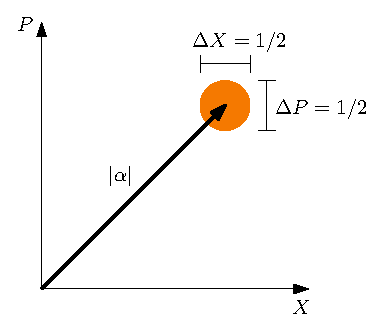
\includegraphics[width=.4\linewidth]{images/coherent_state.eps}
	\caption{Coherent state in phase space. The $x$-axis represents the position and the $y$-axis represents the momentum. To each axis, there is a quantum uncertainty of $1/2$.}
	\label{coherent_state}
\end{figure}
\FloatBarrier

\noindent In Julia with QuantumOptics.jl, we can use the command \texttt{qfunc()} to get the phase space representation of the photon state:

\begin{lstlisting}
bdr = 6
xvec = [-bdr:.1:bdr;]
yvec = [-bdr:.1:bdr;]
photon_dense = ptrace(ψ_states[1], 2)
grid = qfunc(photon_dense, xvec, yvec)
\end{lstlisting}The variable \texttt{bdr} was set heuristically for plotting.